\documentclass[11pt]{article}
\pagestyle{empty}
\usepackage{amsmath,amssymb,amsfonts,setspace,float,enumerate}
\usepackage{graphicx,mathtools}
\usepackage[margin=1in]{geometry}
\usepackage{hyperref}
\usepackage{xcolor}
\usepackage{subcaption}
\hypersetup{
	colorlinks=true,
    linkbordercolor={1 1 1},
    linkcolor = red
}
\parindent 0px
\pagenumbering{gobble}
\singlespacing

\title{Security Cameras Write Up}
\author{David Ye}
\date{\today}

\begin{document}
\maketitle
\section{Linear Program Setup}
All the variables defined in my program are boolean variables. Each boolean variable corresponds to whether or not there is a camera at location $(x,y)$ with direction $(d)$. The boolean variable equals one when there is a camera at the corresponding location and direction, and zero when there is no camera at the corresponding location and direction.

The first constraint is cameras should only be placed adjacent to a wall. To account for this constraint, I only defined boolean variables if the $(x,y)$ location is not on a wall and is neighboring a wall (wall is either left, right, up, or down of $(x,y)$). This way, the linear program only considers camera locations that are feasible, thus cutting down on the number of boolean variables I need to define.

The second constraint is any given $(x,y)$ coordinate should only contain a single camera. To account for this, I defined inequalities such that for every location a camera is allowed, the the sum of all boolean variables at that location (considering cameras of every possible direction) must be less than or equal to one.

The third constraint is every white pixel in the bitmap must lie in the viewable space of at least one camera. To account for this, I first created a list that returned [False] if there is no wall at the specified row and column (i.e. a white pixel) and [True] if there is a wall. Next I created a nested for loop where for every location a camera is allowed, I computed the viewable region of the camera. Wherever the viewable region is True and there is no wall, I appended the boolean variable that represents the camera to the list. For examples, for location $(x,y)$ the list may return $[False, x[x_0,y_0,d_0], x[x_1,y_1,d_1], x[x_2,y_2,d_2]$, where each element after $False$ are boolean variables defined in the linear program. Last but not least, to fullfill the constraint, I wrote a for loop that loops through every white pixel that have cameras that can see it (if no cameras can see a white pixel, then the program skips adding the constraint to avoid no solutions and prints out "no cameras can see this spot") and defined inequalities such that the sum of all boolean variables in the list that correspond to the $(x,y)$ location must be greater than or equal to one (each white pixel must be visible by at least one camera).

\section{Custom Bitmaps}
I designed a few custom bitmaps to compare solving time. I designed a batch of grid-type bitmaps, including bitmaps of 224, 56, 16, and 4 grids. I also designed a circle and square based bitmap. The solving time and total run times are listed in table \ref{table:solvetime}.

Comparing the grids, the total runtime increased as expected as the number of grids increased. This is likely due to the fact there are more walls available for cameras to be placed by, thus more computations of compute viewable are necessary. Unexpectedly, the solving time of the integer program actually increased as the number of grids decreased. This may be because as the number of walls decreases, the white space that need to be covered increases. Thus, more constraints must be added to the integer program. The increase in number of constraints may lead to longer solving times.

Comparing the circle with the square bitmap, the circle bitmap took significantly longer to solve (4800x longer). The circle may have taken much longer because it does not consist of rectangular right angle corners. Rather, a circle is much harder to cover due to its curvature. We can also see in figure \ref{fig:custom} it takes a 18 cameras to cover the circle bitmap, while it only took 7 cameras to cover the square bitmap.

\begin{table}[H]
\centering
\begin{tabular}{|l|l|l|}
\hline
Custom Bitmap & Solving Time (s)& Total Runtime (s)\\ \hline
224 Grid & 1.65 & 1081.59\\ \hline
56 Grid & 2.34 & 1059.87\\ \hline
16 Grid & 3.93 & 970.59\\ \hline
4 Grid & 7.96 & 854.70\\ \hline
Circle & 33125.68 & 34110.51\\ \hline
Square & 6.90 & 1102.20\\ \hline
\end{tabular}
\caption{\label{table:solvetime} Comparing solving time of custom bitmaps from figure \ref{fig:custom}}
\end{table}

Looking at the solved bitmaps in figure \ref{fig:custom}, the cameras are relatively in the correct positions, however in many cases the viewable region of the camera is nonexistent because the camera landed on the wall during up-scaling. Besides camera misplacement, we also see large gaps in coverage of the circle bitmap due to up-scaling.
\begin{figure}[H]%
    \centering
    \subfloat[\centering 4 Grid]{{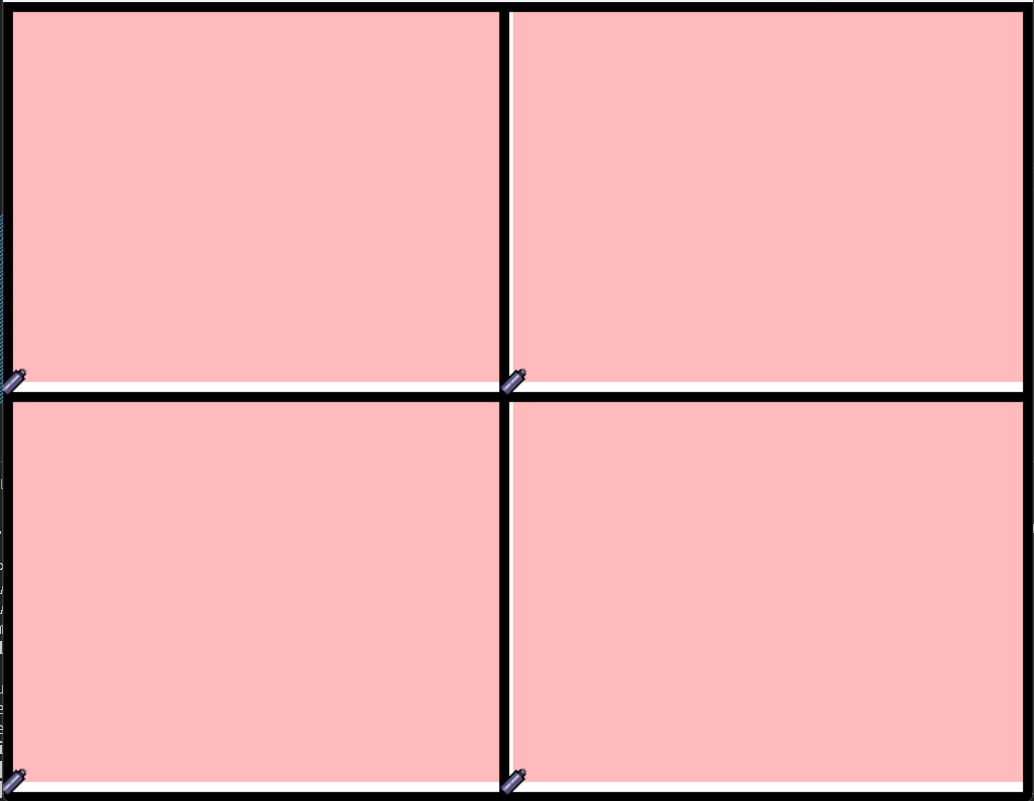
\includegraphics[width=7.5cm]{grid4.png} }}%
    \qquad
    \subfloat[\centering 16 Grid]{{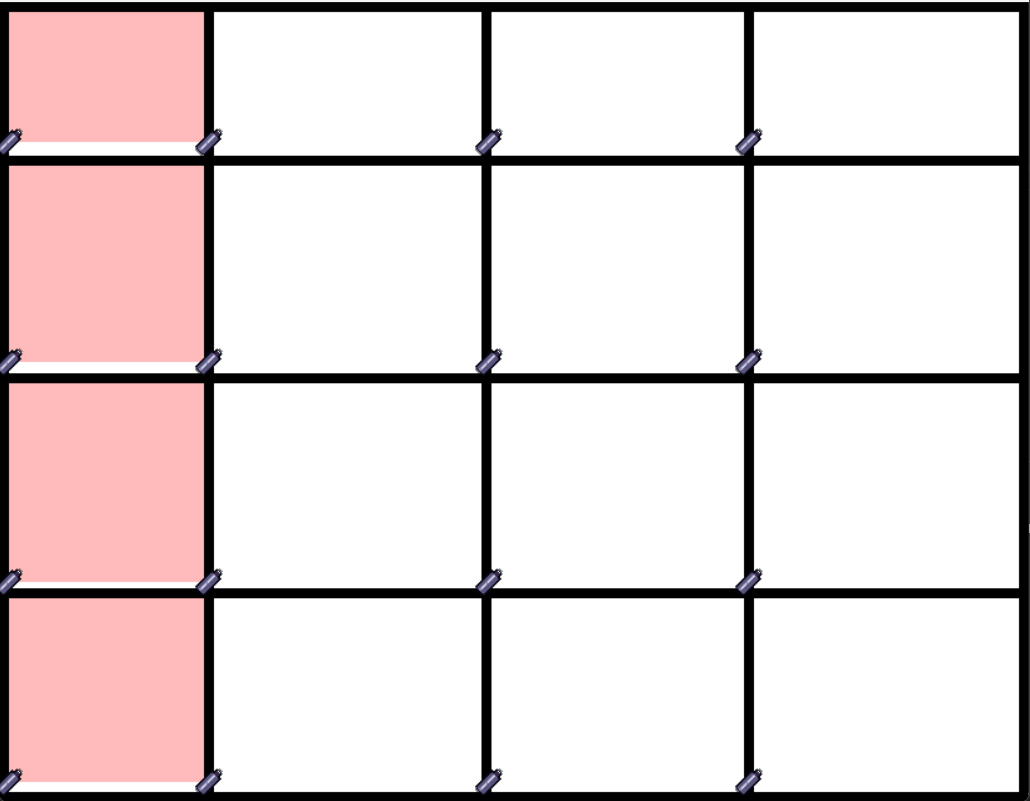
\includegraphics[width=7.5cm]{grid16.png} }}%
    \qquad
    \subfloat[\centering 56 Grid]{{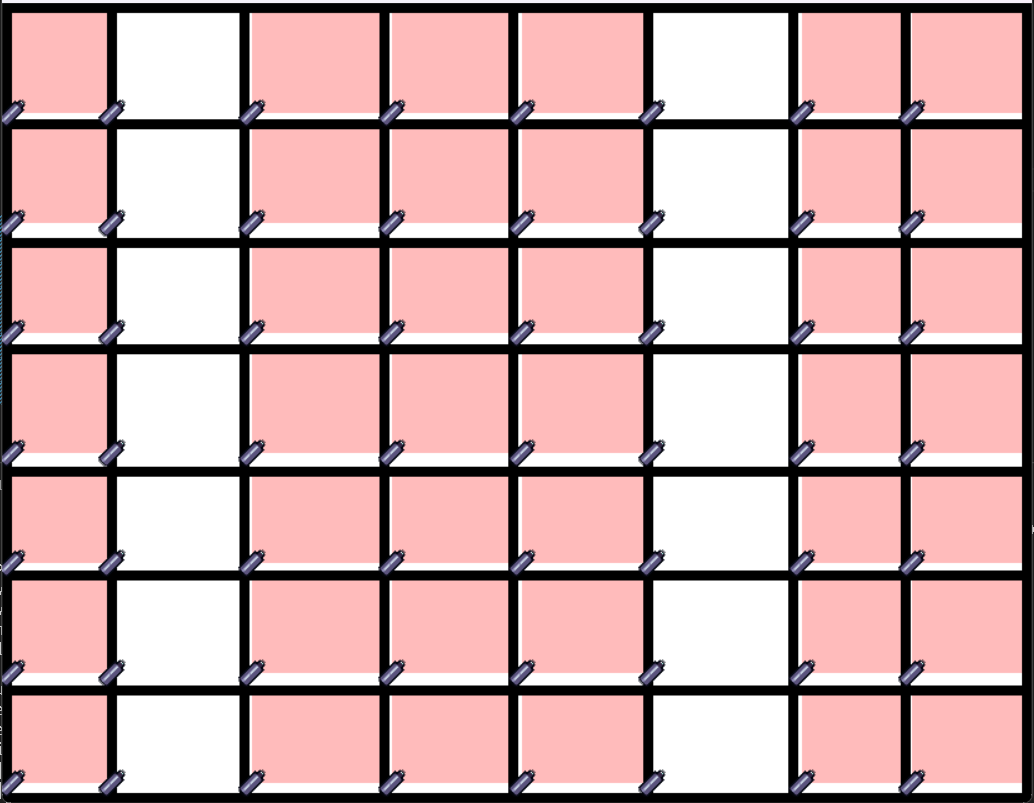
\includegraphics[width=7.5cm]{grid56.png} }}%
    \qquad
    \subfloat[\centering 224 Grid]
{{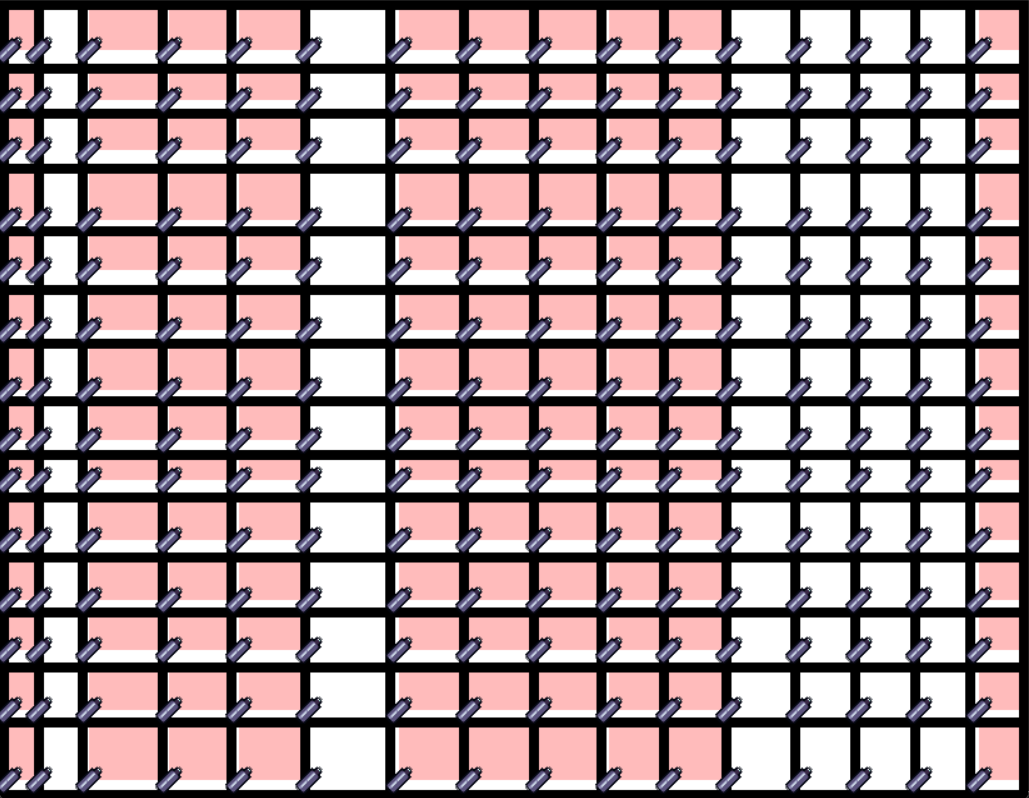
\includegraphics[width=7.5cm]{grid224.png} }}%
    \qquad
    \subfloat[\centering Square]
{{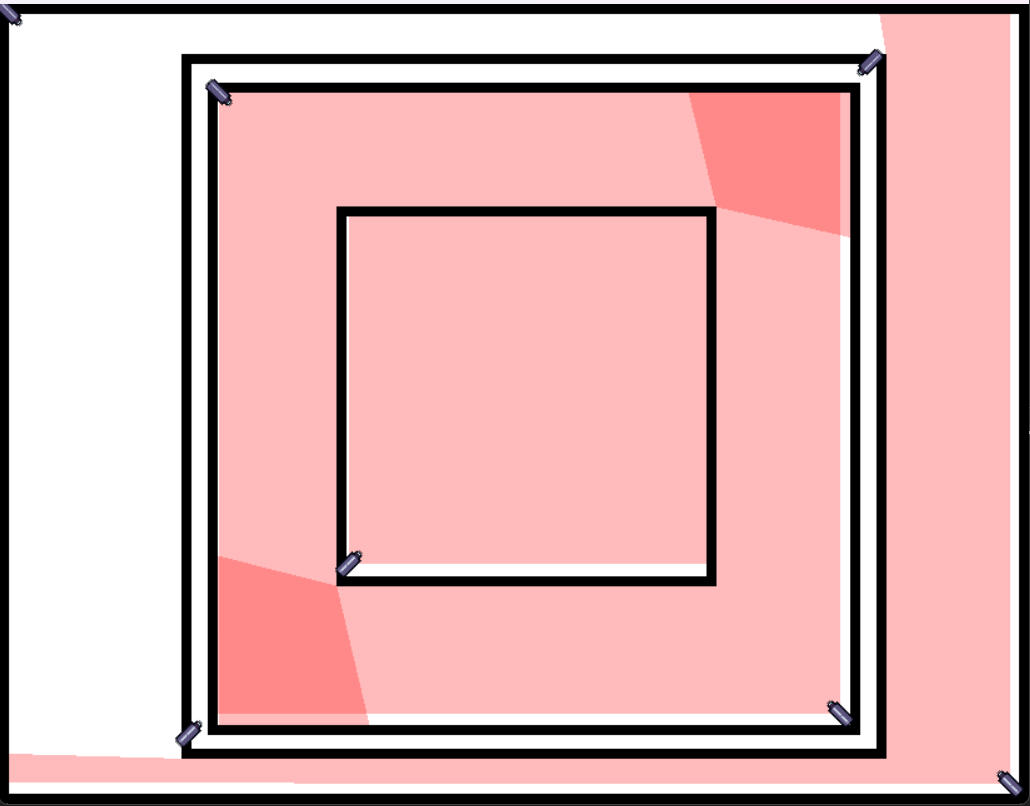
\includegraphics[width=7.5cm]{square.png} }}%
    \qquad
    \subfloat[\centering Circle]  
{{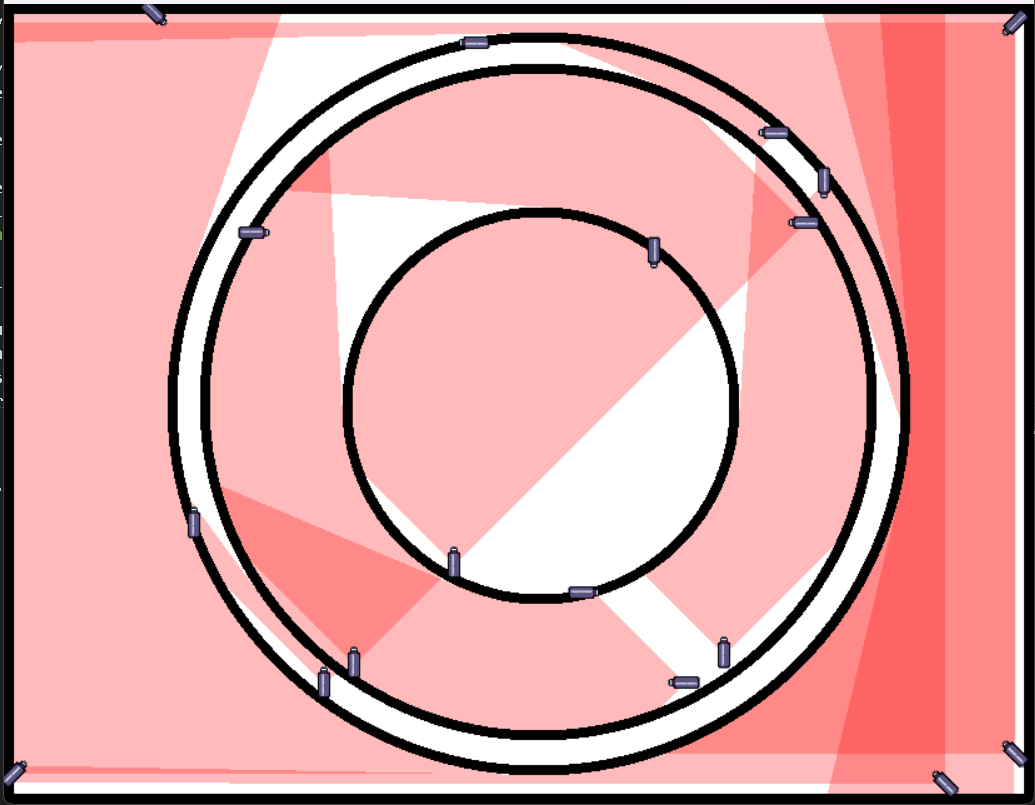
\includegraphics[width=7.5cm]{circle.png} }}%
    \caption{Custom Bitmaps Solved}%
    \label{fig:custom}%
\end{figure}



\section{Manipulating FOV and Number of Directions}
I ran the linear program on a large variety of field of views, from $60^{\circ}$ to $180^{\circ}$ and an additional $360^{\circ}$. The results are shown in table \ref{table:fov}. At $60^{\circ}$, it took 60 cameras to completely cover the museum. As the FOV increased, the number of cameras needed to cover the museum decreased. The largest decrease in number of cameras needed to cover museum occured between $80^{\circ}$ and $90^{\circ}$ FOV cameras. The number of cameras needed dropped from 52 down to 36 (dropped 16 cameras). This huge drop can be seen in graph \ref{fig:graph}. As the FOV increased past $90^{\circ}$, the number of cameras needed dropped very slowly. In fact, between $110^{\circ}$ and $170^{\circ}$, the number of cameras needed steadily remained at 34 (only two cameras less than $90^{\circ}$). Finally, with the best possible FOV of $360^{\circ}$, the number of cameras dropped down to 30. From this analysis, it may be most effective to purchase cameras with at least $90^{\circ}$ FOV. However, going above $90^{\circ}$ does not reduce the number of cameras needed by much.
\begin{table}[H]
\begin{tabular}{|l|l|l|l|l|l|l|l|l|l|l|l|l|l|l|}
\hline
Floor & $60^{\circ}$ & $70^{\circ}$& $80^{\circ}$& $90^{\circ}$ & $100^{\circ}$& $110^{\circ}$& $120^{\circ}$& $130^{\circ}$& $140^{\circ}$& $150^{\circ}$& $160^{\circ}$& $170^{\circ}$& $180^{\circ}$& $360^{\circ}$\\ \hline
1 & 30 & 27& 26&19&18 & 17&17&17&17&17&17&17&17&15\\ \hline
2 & 16 & 14& 14&9&9 & 9&9&9&9&9&9&9&9&8\\ \hline
3 & 14 & 13&12&8 & 8&8&8&8&8&8&8&8&7&7\\ \hline
Total & 60 & 54&52&36&35&34&34&34&34&34&34&34&33&30\\ \hline
\end{tabular}
\caption{\label{table:fov} Comparing minimum number of cameras needed to cover all floors of the museum for a variety of field of view angles}
\end{table}

\begin{figure}[H]
	\centering
	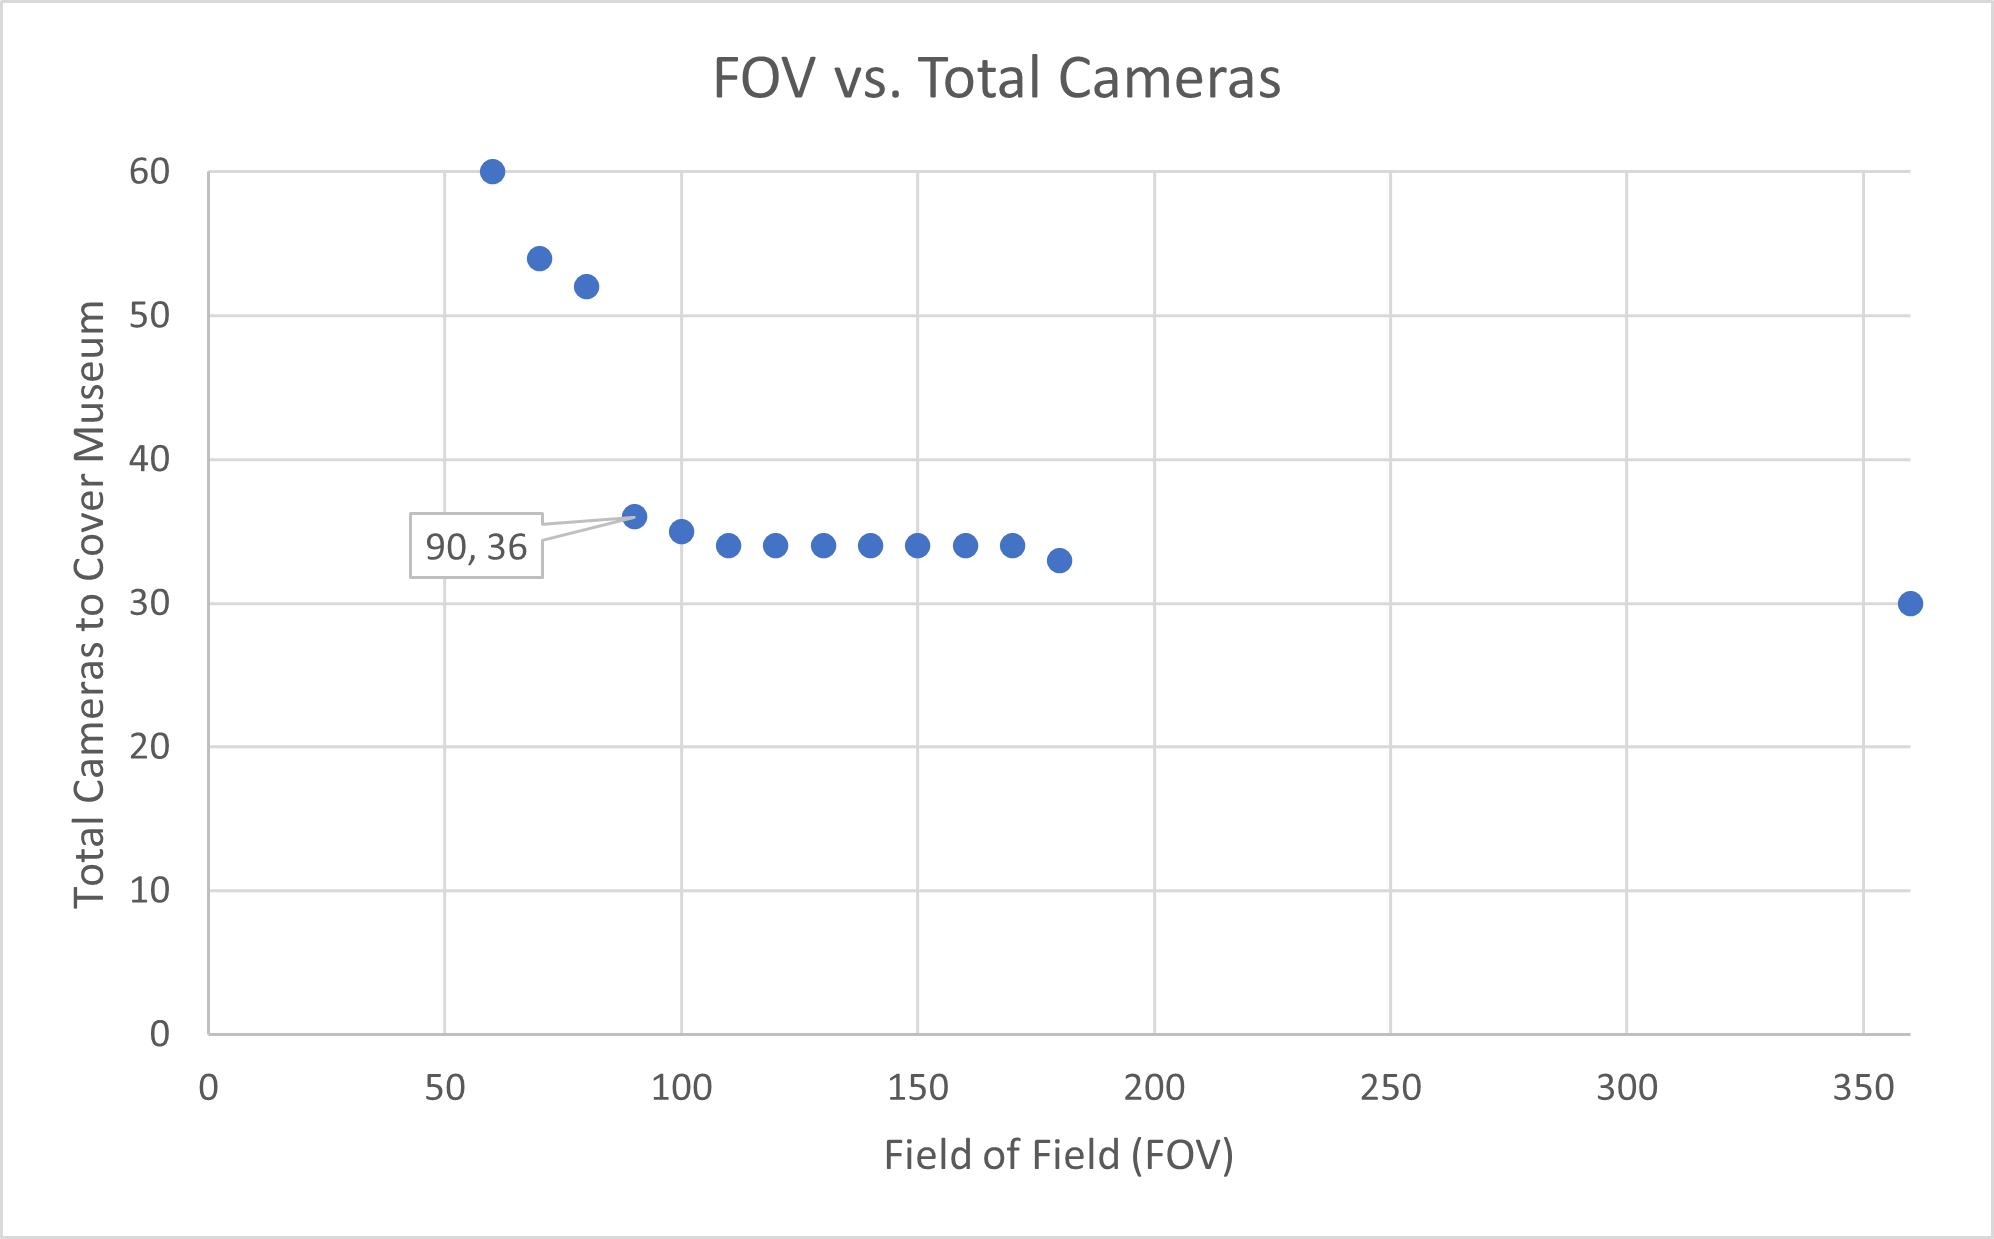
\includegraphics{graph.png}
	\caption{\label{fig:graph} On the x-axis is the cameras' field of view and on the y-axis is the total number of cameras needed to cover all three levels of the museum}
\end{figure}

\section{Possible Improvements}
Something interesting to note is the locations computed on the down-scaled images may not work on the up-scaled images. For example, in floor two the Raphael Room is not in complete view because the camera meant to view Raphael room ended up on the wall (from up-scaling) rather than adjacent to it. The simplest solution would be to move the misplaced camera to the right until it is no longer on the wall. Another possible approach could be to move all computed cameras to their closest corner (camera adjacent to two walls). This approach would reduce camera misplacement as well as remove the visible buffer between the wall and the camera's view. However, this approach is limited to rectangular floor/room designs and may not give correct results. It would be wise to compare the results of post-processing with the original up-scaled image without post-processing to ensure no cameras were severely misplaced.
\begin{figure}[H]
	\centering
	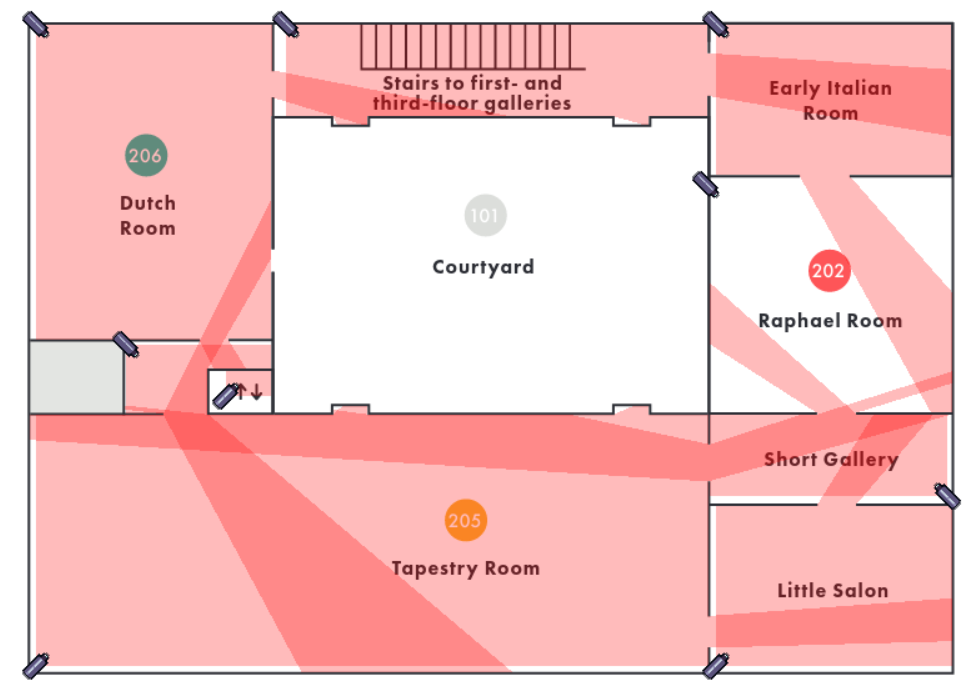
\includegraphics[width=7.5cm]{Floor2_90.png}
	\caption{\label{fig:visited_show} Camera that should cover Raphael Room is misplaced on the wall}
\end{figure}

\end{document}